
\setcounter{secnumdepth}{4}

\titleformat{\paragraph}
{\normalfont\normalsize\bfseries}{\theparagraph}{1em}{}
\titlespacing*{\paragraph}
{0pt}{3.25ex plus 1ex minus .2ex}{1.5ex plus .2ex}

%--------------------------------------------------------------------------------
\section{Prior Work}

Prediction of stock prices is the famous problem for several years now. In the era of deep learning various researchers have done the contribution to this topic. Hao Li et al. (2018)\cite{} proposed a Attention based Multi Input LSTM for prediction of opening price given the historical values. It uses attention mechanism for noise filtering and extracting the related information from related stocks. Yao Qin et al. (2017)\cite{} proposed a dual attention based RNN for prediction of treading index using the historical prices of 81 different stocks. The dual attention consists of the input attention mechanism for encoder and a temporal attention mechanism for decoder. Rather et al. (2015)\cite{} proposed the hybrid approach containing RNN and statistical models for prediction of stock price. 

%--------------------------------------------------------------------------------
\section{Algorithm}

The data is collected prior from 2013 to 2018 for the historical stock price of Infosys stock named INFY. The algorithm is trained on the 90\% of the data and tested on the rest of the 10\% of the data. The algorithm is as follows:

\begin{itemize}
		
\item \textbf{Task: } Prediction of Stock Price
			
\item \textbf{Data: } \{X\textsubscript{i} : Open\textsubscript{i}, High\textsubscript{i}, Low\textsubscript{i} ; Y\textsubscript{i} : Close\textsubscript{i} \}$_{i =1}^{N}$		%\textsubscript{i = 1}\textsuperscript{N}
			
\item \textbf{Model: } LSTM: \begin{equation} h_{t}, C_{t} = LSTM(h_{t-1}, C_{t-1}, X_{t}) \end{equation} 	
			
\item \textbf{Parameters: } W$_{f}$, b$_{f}$, W$_{i}$, b$_{i}$, W$_{c}$,  b$_{c}$, W$_{o}$, b$_{o}$ 

\item \textbf{Loss Function: } \begin{equation}Mean Squared Error (MSE) =  \frac{1}{n}\Sigma_{i=1}^{n} (Predicted\_Y_{i} - Y_{i})^2 \end{equation}

\item \textbf{Algorithm: } Adam is the algorithm used for learning the parameters for the LSTM model.


\begin{algorithm}[H]

\caption{Learning Parameters of LSTM for Prediction of Stock Price}

\begin{algorithmic}[1] 
						
\STATE Parameter Initialization: \{strategy = Uniform\} 

\STATE $\emph{epoch} \gets Positive\_Integer$

\STATE \emph{while(eopch > 0)}:

\STATE \tab	Forward Propagation of Data in Model

\STATE \tab	Compute Loss using Loss Function

\STATE \tab	Compute Gradients with respect to Loss

\STATE \tab	Update the Parameters in Backward Propagation	

\STATE\tab	$\emph{epoch} \gets \emph{epoch}-1$

\end{algorithmic}

\end{algorithm}

\end{itemize}

%-----------------------------------------------------------------------------------------------------------------------------
\section{Illustration}
%\paragraph{}
The experimental setup was done in Google Colab, a facility provided by Google Inc. to students and researchers for training deep learning algorithms where they provide free GPU. The computational specification of Colab is as follows:
\begin{itemize}
\item CPU model name: Intel(R) Xeon(R) CPU @ 2.30GHz  
\item No. of Processors : 2
\item CPU Cache Size : 46080 KB
\item GPU Name : Tesla T4
\item GPU Memory : 16 GB (15079MiB usble)
\item RAM : 12.9 GB
\end{itemize}

%\paragraph{}
The programming language used for performing experiment is Python 3.6. The packages used for the experiment include sklearn, keras, math, time, pandas, numpy, pandas\_datareader, matplotlib, h5py,statsmodels, etc.

The hyper-parameters that were fine tuned during the experiment for better performance of the model are as follows with their fine tuned values:

\begin{itemize}

\item seq\_len = 22		\# Input Window Size

\item shape = [4, seq\_len, 1] 	\# No. of Features, Window, Output

\item epochs = 90 		\# No. of times the the forward and backward propagation happens on whole training data through the model

\item dropout rate = 0.3 		\# that percent of neurons from the model will be dropped for each epoch randomly

\item decay = 0.2 		\# parameter decay rate for Adam optimizer

\item neurons = [512, 512, 64, 1]	\# the different combinations of neurons is tried for optimization


\end{itemize}

%\paragraph{}
The architecture of the model used for experimentation is as follows:

%				\begin{center}
%				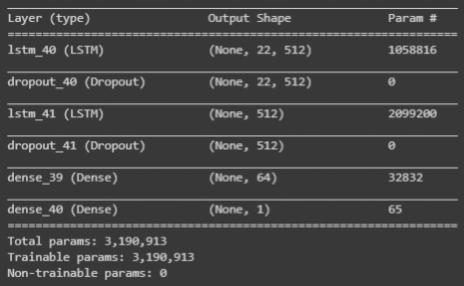
\includegraphics[width=\linewidth]{figures/Model-Sumary.jpg}	
%				\captionof{figure}{The architecture of the LSTM model}
%				\label{fig: The architecture of the LSTM model}
%				\end{center}


\begin{table}[h!]
  \begin{center}
    \caption{The architecture of the LSTM model}
    \label{tab:The architecture of the LSTM model}
    \begin{tabular}{l|l|l} % <-- Alignments: 1st column left, 2nd middle and 3rd right, with vertical lines in between
      \hline
      \textbf{Layer (type)} & \textbf{Output Shape} & \textbf{Param \#}\\
	\hdashline
	\hdashline
      lstm\_40 (LSTM) & (None, 22, 512) & 1058816\\
	\hline
      dropout\_40 (Dropout) &  (None, 22, 512) & 0\\
	\hline
      lstm\_41 (LSTM) & (None, 512) & 2099200 \\
	\hline
      dropout\_41 (Dropout) & (None, 512) & 0 \\
	\hline
      dense\_39 (Dense) & (None, 64) & 32832 \\
	\hline
      dense\_40 (Dense) & (None, 1) & 65 \\
	\hdashline
	\hdashline
	\multicolumn{3}{l}{Total params: 3,190,913} \\
	\multicolumn{3}{l}{Trainable params: 3,190,913} \\
	\multicolumn{3}{l}{Non-trainable params: 0} \\
	\hline
    \end{tabular}
  \end{center}
\end{table}


%\end{itemize}
				\begin{center}
				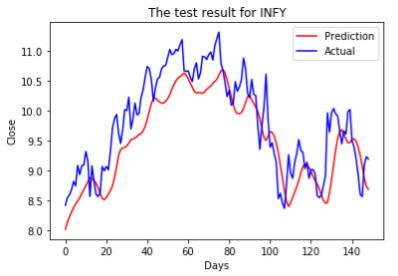
\includegraphics[width=\linewidth]{figures/test-data-results.jpg}	
				\captionof{figure}{Plot showing of Actual and Predicted values}
				\label{fig: Plot showing of Actual and Predicted values}
				\end{center}

%--------------------------------------------------------------------------------
\section{Computational Complexity}

Computational complexity of LSTM is O(Z),\\
  where Z = 4 * \#IP * h + 4 * h$^{2}$ + 3 * h + h * \#OP , \\
 \tab\#IP: Number of inputs\\
 \tab\#h: Number of hidden layers\\
 \tab\#OP: Number of outputs\\

The total time taken by the model to train is 1min 9 sec.
%--------------------------------------------------------------------------------
\section{Comparative Analysis} 

After training the LSTM model we have tested the model on unseen test data and the MSE is as follows:
\begin{itemize}
\item MSE on Train Data: 0.00128 MSE
\item MSE on Test Data: 0.00230 MSE

The predictions of ARIMA and Auto-ARIMA models were taken into consideration for comparison with predictions of LSTM model. 
\begin{itemize}
\item MSE on Test Data of ARIMA Model:  0.576 MSE
\item MSE on Test Data of Auto-ARIMA Model:  0.695 MSE
\end{itemize}
				\begin{center}
				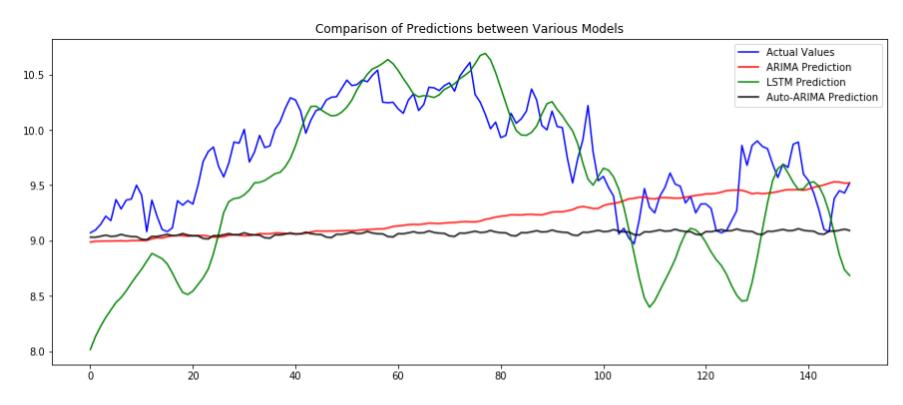
\includegraphics[width=\linewidth]{figures/Comp-ARIMA-LSTM.jpg}	
				\captionof{figure}{Comparison of Prediction between ARIMA Model and LSTM Model with Actual Values}
				\label{fig: Comparison of Prediction between ARIMA Model and LSTM Model with Actual Values}
				\end{center}
\end{itemize}
%--------------------------------------------------------------------------------
\section{Conclusion }

In this chapter we have discussed about the model architecture, its parameters, and tuning the parameters for optimization of performance of the model. The LSTM model performed far better than the statistical models.
